\chapter{State Of The Art}

Since there was no similar comparison about LD frameworks found, this section will 
cover general comparisons of frameworks in the field of semantic web.

\section{Benchmarking Database Representations of RDF/S Stores}

Theoharis et. al. conducted a benchmark in their paper \emph{Benchmarking Database 
Representations of RDF/S Stores} (~\cite{theoharis2005benchmarking}) in order to 
compare different kind of RDF stores. They examined three popular database 
representations of RDF/S schemata and data: schema-aware, with explicit (ISA) or 
implicit (NOISA) storage of subsumption relationships, schema-oblivious using (ID) 
or not (URI) identifiers to represent resources and hybrid of the schema-aware and 
schema-oblivious representations. Further, they benchmarked two common approaches 
for evaluating taxonomic queries : on-the-fly (ISA, NOISA, Hybrid) and by 
precomputing the transitive closure of subsumption relationships (MatView, URI, 
ID). 

"The main conclusion drawn is that the evaluation of taxonomic queries is most 
efficient over RDF/S stores utilizing the Hybrid and MatView representations. Of 
the rest, schema-aware representations (ISA, NOISA) exhibit overall better 
performance than URI, which is superior to that of ID, which exhibits the overall 
worst performance."(~\cite{theoharis2005benchmarking})

\section{Ontology Alignment Evaluation Initiative (OAEI)}

Since 2004 the initiative organizes every year evaluations of various ontology 
matching systems. The official result are published on their website~
\footnote{\url{http://oaei.ontologymatching.org/}}. There are also a various kind 
of papers available, analyzing the outcome of the evaluations, the last ones are 
from 2016 (\cite{achichi2016results}), 2015 (\cite{cheatham2015results}) and 2014 
(\cite{dragisic2014results}). The results of 2017 are not available at the point 
of writing this thesis.

In order to evaluate a benchmark, the initiative provides a set of test cases, 
ranging from real world cases to generated cases. Participants register their 
tools themselves, which then will be run by the organizers with both blind and 
published datasets. The evaluation then uses the SEALS infrastructure since 2011 
and is since 2006 usually reported at the Ontology matching workshop of the 
International Semantic Web Conference.

\section{Quality Assessment for Linked Data: A Survey}

Aim of Zaeri et. al in their survey~\cite{zaveri2016quality} was a systematic 
review of approaches for assessing the quality of LD, since they observed "widely 
varying data quality ranging from extensively curated datasets to crowdsourced and 
extracted data of relatively low quality". Their goal was to obtain an 
understanding of the differences of existing approaches. They gathered these 
approaches and analyzed them qualitatively, providing a list of 18 quality 
dimensions (grouped by accessibility, intrinsic, contextual and representational) 
and 69 metrics. Furthermore, they analyses 30 core approaches and 12 tools using a 
set of attributes.

As result, they observed that "this research area is still in its infancy and can 
benefit from the possible re-use of research from mature, related domains. 
Additionally, in most of the surveyed literature, the metrics were often not 
explicitly defined or did not consist of precise statistical measures."

\section{An Evaluation Framework For Spreadsheet Tools Comparison}

In the paper \emph{Towards Evaluation and Comparison of Tools for Ontology 
Population from Spreadsheet Data} by Kovalenko et al (\cite{kovalenko2013towards}) 
an evaluation framework was proposed by the authors in order to facilitate tools 
comparison, mainly for Ontology Population from Spreadsheet Data but also 
applicable for other comparisons. They analyzed different types of end users 
(Semantic Web Experts, Domain Experts and Software Developers) and their needs as 
well as performed a literature analysis on Tools for Ontology Population from 
Spreadsheet Data. The result are the following criteria:

\begin{itemize}
\item \textbf{(C1) General Information} with \textit{Maturity}, \textit{License} and \textit{Type} as sub criteria
\item \textbf{(C2) Usability} with \textit{GUI} and \textit{Required User Knowledge} as sub criteria
\item \textbf{(C3) Input format}
\item \textbf{(C4) Output format}
\item \textbf{(C5) Mappings} with \textit{Internal Representation}, \textit{External Representation} and \textit{Storage} as sub criteria
\item \textbf{(C6) Expressiveness}
\item \textbf{(C7) Multi-user support}
\item \textbf{(C8) Required software}
\item \textbf{(C9) Additional features}
\end{itemize}

This criteria can used not only for comparison but also for classification of 
tools as well as for a search for an appropriate tool for a specific task/problem. 
In order to prove the usefulness, the authors performed a qualitative analysis and 
comparison of a representative set of seven tools (\textbf{RDF123, XLWrap, Mapping 
Master, Populous, Anzo for Excel, TopBraid, Google Refine}). 

\section{The Berlin SPARQL Benchmark}

In the article \textit{The Berlin SPARQL Benchmark} (BSBM) by Bizer and Schultz 
(\cite{bizer2009berlin}) the authors introduced a benchmark for comparing 
performance of native RDF stores with the performances of SPARQL-to-SQL rewriters 
across architectures. The benchmark query simulates the search and navigation 
pattern of a consumer looking for a product, representing an e-commerce use case. 
The article presents, next to the discussion about the benchmark itself, results 
of the benchmark including for popular RDF stores (\textbf{Sesame}, 
\textbf{Virtuoso}, \textbf{Jena TDB} and \textbf{Jena SDB}) as well as two SPARQL-
to-SQL rewriters (\textbf{D2R Server} and \textbf{Virtuoso RDF Views}) and 
relational database management systems (\textbf{MySQL} and \textbf{Virtuoso 
RDBMS}). An excerpt of the result can be seen in figure~\ref{bsbm_sample}.

\begin{figure}[htbp]
	\centering
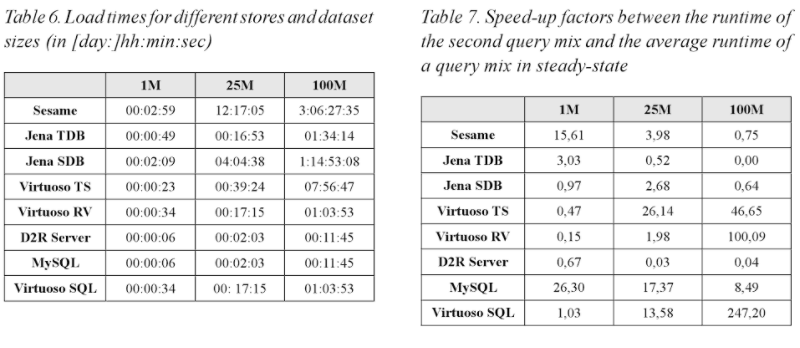
\includegraphics[width=\textwidth]{img/bsbm_sample.png}
	\caption{Excerpt of the Berlin SPARQL Benchmark results}
	\label{bsbm_sample}
\end{figure}

\section{Benchmarking Fulltext Search Performance of RDF Stores}

Another benchmark in the area of semantic web (next to many others) is the 
benchmark proposed by Minack et al in their paper \textit{Benchmarking Fulltext 
Search Performance of RDF Stores} (\cite{minack2009benchmarking}). They extended 
the existing LUBM benchmark with "synthetic scalable fulltext data and 
corresponding queries for fulltext-related query performance evaluation". The 
benchmark was then applied to four popular RDF stores (\textbf{Jena}, 
\textbf{Sesame2}, \textbf{Virtuoso}, and \textbf{YARS}). An excerpt of the result 
can be seen in figure~\ref{minack_sample}.

\begin{figure}[htbp]
	\centering
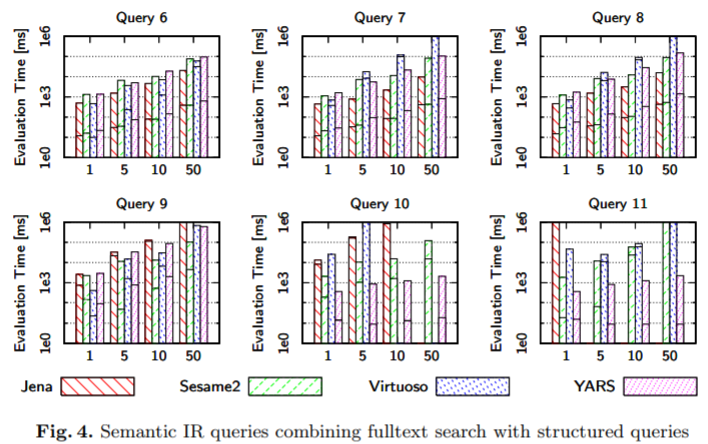
\includegraphics[width=\textwidth]{img/minack_sample.png}
	\caption{Excerpt of the Berlin SPARQL Benchmark results}
	\label{minack_sample}
\end{figure}